\graphicspath{{./chapters/chapter0/}}
\chapter{Appendix for Chapter 1}
\section{Proofs for $r$-separated distributions}

For any distribution $\D$ over $\X \times Y$, it will be convenient to use the following notation: for any measurable $S \subset \X$, let $\P_\D[S] = \P_{(x,y) \sim \D}[x \in S]$. The following definition will be central to our proofs. 

\begin{defn}
Let $\D$ be a distribution over $\X \times Y$. An \textbf{$(\epsilon, \gamma, \alpha)$-decomposition} of $\D$ is a finite set of closed balls $B_1, B_2, \dots, B_s \subset \X$ each with radius $\gamma$ such that $$\P_\D[\cup_1^s B_i] > 1 - \epsilon,$$ and such that $\P_\D[B_i] \geq \alpha > 0$ for $1 \leq i \leq s$. 
\end{defn}


\begin{lem}\label{lem_balls}
Let $\X$ be a totally bounded metric space. For any distribution $\D$, and $\epsilon, \gamma > 0$, there exists $\alpha > 0$ such that $\D$ admits a $(\epsilon, \gamma, \alpha)$-decomposition. 
\end{lem}

\begin{proof}
Fix any $x \in \X$ and $\epsilon, \gamma > 0$. Then the sequence of balls $\{S_i = B(x, i)\}$ has union equal to $\X$. Therefore, there exists $j$ such that $P_\D(S_j) > 1 - \epsilon$. Since $S_j$ is totally bounded and complete, it is compact. Let $B^o(x, a)$ denote the open ball centered at $x$ with radius $a$. Therefore, taking an open cover of $S_j$, $\{B^o(x, \gamma): x \in S_j\}$, we can take a finite subcover $\{B_1^o, B_2,^o, \dots, B_t^o\}$ that cover $S_j$. Discarding balls such that $\P_\D(B_i^o) = 0$ and taking the closure of each ball gives the desired result, with $\alpha = \min_{i}P_\D(B_i)$.  
\end{proof}

To prove Theorem \ref{thm_stone_cons}, we use the following lemma. 

\begin{lem}\label{lem_expectation}
Let $\D$ be a distribution over $\X \times \Y$, and let $B_1, B_2, \dots, B_s$ be a $(\epsilon, \gamma, \alpha)$-decomposition of $\D$, and let $r > 3\gamma$. If $W$ is a weight function satisfying the conditions of Theorem \ref{thm_stone_cons}, then for any $\delta > 0$ there exists $N$ such that for $n \geq N$, with probability $1-\delta$ over $S \sim \D^n$, and $w_1, w_2, \dots, w_n$ learned by $W$ from $S$, $$\sup_{\{x: d(x, \cup_1^s B_i) \leq r - 3\gamma\}} \sum_1^n w_i(x)I_{d(x_i, x) > r} < \frac{1}{3}.$$
\end{lem}

\begin{proof} 
Fix $\delta > 0$, and let $Y$ be the indicator variable defined as $$Y = \begin{cases} 1 & \text{ if }\sup_{\{x: d(x, \cup_1^s B_i) \leq r - 3\gamma\}} \sum_1^n w_i(x)I_{d(x_i, x) > r} \geq \frac{1}{3} \\ 0 & \text{ if }\sup_{\{x: d(x, \cup_1^s B_i) \leq r - 3\gamma\}} \sum_1^n w_i(x)I_{d(x_i, x)> r} < \frac{1}{3} \end{cases}.$$ It suffices to show that there exists $N$ such that for all $n \geq N$, $E_{S \sim \D}[Y] \leq \delta$. 

Fix $S \sim \D^n$ and suppose that $Y = 1$. Then there exists $x^*, B_i^*$ such that $d(x^*, B_i^*) \leq r - 3\gamma$ and such that $$\sum_1^n w_i(x^*)I_{d(x_i, x^*) > r} \geq \frac{1}{3}.$$ By definition, $B_i$ has radius $\gamma$, so by the triangle inequality, for any $x \in B_i^*$, $d(x, x^*) \leq 2\gamma + r - 3\gamma = r - \gamma$. This implies $x^* \in B(x, r-\gamma)$. Therefore, for any $x \in B_i^*$, $$\sup_{x' \in B(x, r-\gamma)} \sum_1^n w_i(x')I_{d(x', x_i) > r} \geq \sum_1^n w_i(x^*)I_{d(x^*, x_i) > r} \geq \frac{1}{3}.$$ By the definition of an $(\epsilon, \gamma, \alpha)$-decomposition, we have that $P_\D(B_i^*) \geq \alpha$. As a consequence, we have that $$\mathbb{E}_{X \sim \D_\X} \big [ \sup_{x' \in B(X, r-\gamma)} \sum_1^n w_i(x')I_{||x_i - x'|| > r} \big] \geq P_\D[B_i^*]\frac{1}{3} \geq \frac{\alpha}{3}.$$ Since the previous inequality is guaranteed to hold if $Y = 1$, taking the expectation over $S$ yields that $$\mathbb{E}_{S \sim \D^n} \mathbb{E}_{X \sim \D_\X} \big [ \sup_{x' \in B(X, r-\gamma)} \sum_1^n w_i(x')I_{||x_i - x'|| > r} \big] \geq \frac{\alpha E[Y]}{3}.$$ By the conditions of Theorem \ref{thm_stone_cons}, the left side of the equation must tend to $0$ as $n \to \infty$. This implies that the same must hold for the right side. Therefore, $E[Y]$ tends to $0$ as $n \to \infty$, and we can select $N$ such that $E[Y] < \delta$ for $n \geq n$, which completes the proof. 
\end{proof}

\begin{proof} (\textbf{Theorem \ref{thm_stone_cons}})
Let $W$ be a weight function that satisfies the condition of Theorem \ref{thm_stone_cons}. Fix $\epsilon, \delta > 0$, and $\gamma < r/3$. Applying Lemma \ref{lem_balls}, let $B_1, B_2, \dots, B_s$ be an $(\epsilon, \gamma, \alpha)$-decomposition of $\D$. Let $T^+$ and $T^-$ be subsets of $\X$ corresponding to the definition of $r$-separation for $\D$.  

For $S \sim \D^n$, let $A$ denote the event that $$\sup_{\{x: d(x, \cup_1^s B_i) \leq r - 3\gamma\}} \sum_1^n w_i(x)I_{d(x_i, x) > r} < \frac{1}{3}.$$
Suppose $A$ holds. Pick a $B_i$. Since $T^+$ and $T^-$ have distance greater than $2r$, and $diam(B_i) \leq 2\gamma < r$, either $B_i \cap T^+ = \emptyset$ or $B_i \cap T^- = \emptyset$. Note that for $n$ sufficiently large, both cannot be empty since $P_\D(B_i) \geq \alpha > 0$ and each $x$ in the support of $\D$ is either in $T^+$ or $T^-$. 

Without loss of generality, $B_i \cap T^- = \emptyset$. Then $B_i \cap T^+ \neq \emptyset$. $B_i$ has diameter $2\gamma$. Thus $d(B_i, T^-) > 2r - 2\gamma$. Let $x \in B(B_i, r-3\gamma)$. Then if $(x_j, -) \in S$, by the triangle inequality, $d(x, x_j) > 2r -2\gamma - (r - 3\gamma) = r+\gamma$. 

Substituting this and using event $A$, we have that $$\sum_1^n w_i^S(x)I_{(x_i, -) \in S} \leq \sum_1^n w_i^S(x)I_{d(x_i, x) > r} < \frac{1}{3}.$$ It follows that $W_S(x) = +1$. An analogous argument holds for $B_i \cap T^+ = \emptyset$. This implies that $W_S$ is astute with radius $r-3\gamma$ over all $B_i$.

$\cup B_i$ has measure at least $1-\epsilon$. By Lemma \ref{lem_expectation}, for any $\delta>0$ event $A$ holds with probability $1-\delta$ for $n$ sufficiently large. Therefore, for $n$ sufficiently large, we see that $A_{r-3\gamma}(W_S, \D) \geq 1-\epsilon$ with probabiltiy $1-\delta$. Because $\epsilon, \delta$ and $\gamma$ were arbitrary, it follows that $W$ is \rcons,\emph{ }as desired.

\end{proof}

\begin{proof} (\textbf{Corollary \ref{nn_sep_thm}})
For any $S = \{(x_1, y_1), (x_2, y_2), \dots, (x_n, y_n)\} \subset \X \times \Y$, let $w_i^S(x)$ be $1$ if and only if $x_i$ is one of the $k_n$ nearest neighbors of $x$ in the set $S_\X = \{x_1, x_2, \dots x_n\}$. Let $\D$ be a distribution over $\X \times \Y$. By Theorem \ref{thm_stone_cons}, it suffices to show that for any $0 < a < b$, $$\lim_{n \to \infty} \mathbb{E}_{X \sim \D_\X}[\mathbb{E}_{S \sim \D^n} [\sup_{x' \in B(x,a)} \sum_1^n w_i^S(x')I_{d(x_i, x') > b}]] = 0.$$ Fix $0 < a < b$, and let $\epsilon > 0$. 

Pick $\gamma > 0$ such that $a+ 2\gamma < b$. This is possible for any $a < b$. Let $B_1, B_2, \dots, B_s$ be an $(\epsilon, \gamma, \alpha)$-decomposition of $\D$. By applying a Chernoff bound followed by a union bound, for any $\delta > 0$ there exists $n$ such that with probability $1-\delta$ over $S \sim \D^n$, each $B_i$ satisfies $|B_i \cap S_\X| \geq \frac{n\alpha}{2}$. Furthermore, if $n$ is sufficiently large, then $\frac{n\alpha}{2} > k_n$ holds as well. 

Consider any $x \in B_i$, and$x' \in B(x,a)$. $B_i$ has radius $\gamma$ and also satisfies $|B_i \cap S_\X| > k_n$. Therefore, there are at least $k_n$ points within distance $a+2\gamma$ of $x$. Because $a + 2\gamma < b$, it follows that none of the $k_n$ nearest neighbors of $x'$ can have distance more than $b$ from $x'$. In particular, $$\sum_1^n w_i^S(x')I_{d(x_i, x') > b} = 0.$$ Since $B_i$, $x$ and $x'$ were arbitrary, we have that for all $x \in \cup B_i$, $$\sup_{x' \in B(x,a)} \sum_1^n w_i^S(x')I_{d(x_i, x') > b} \leq  \begin{cases} 0 & |B_i \cap S_\X| \geq \frac{n\alpha}{2}, 1 \leq i \leq s \\ 1 & \text{otherwise} \end{cases}$$

Since $X \in \cup_1^s B_i$ with probability at least $1-\epsilon$, and since $|B_i \cap S_\X| \geq \frac{n\alpha}{2}, 1 \leq i \leq s$ with probability at least $1-\delta$, it follows that $$\mathbb{E}_{X \sim \D}[\mathbb{E}_{S \sim \D^n} [\sup_{x' \in B(x,a)} \sum_1^n w_i^S(x')I_{d(x_i, x') > b}]] \leq (1- \delta - \epsilon)0 + \delta + \epsilon = \delta + \epsilon,$$ which can be made arbitrarily small as $\epsilon$ and $\delta$ were arbitrary. Therefore, the limit as $n$ approaches infinity is $0$, as desired.
\end{proof}

\begin{proof} (\textbf{Corollary \ref{thm_kernel}})
Let $\D$ be a distribution over $\X \times \Y$. By Theorem \ref{thm_stone_cons}, it suffices to show that for any $0 < a < b$, $$\lim_{n \to \infty} \mathbb{E}_{X \sim \D}[\mathbb{E}_{S \sim \D^n} [\sup_{x' \in B(x,a)} \sum_1^n w_i^S(x')I_{d(x_i, x') > b}]] = 0.$$ Fix $0 < a < b$, and let $\epsilon > 0$. 

Pick $\gamma > 0$ be such that $a+ 2\gamma < b$. Let $B_1, B_2, \dots, B_s$ be an $(\epsilon, \gamma, \alpha)$-decomposition of $\D$. By applying a Chernoff bound, for any $\delta > 0$ there exists $n$ such that with probability $1-\delta$ over $S \sim \D^n$, each $B_i$ satisfies $|B_i \cap S_\X| \geq \frac{n\alpha}{2}$.

Next, consider any $x_i, x_j \in S_\X$, and let $x$ be a point such that $d(x_i, x) \leq a+2\gamma$ and $d(x_j, x) > b$. Then we have that 
\begin{equation*}
\begin{split}
\frac{w_j^S(x)}{w_i^S(x)} = \frac{K(\frac{d(x_j, x)}{h_n})}{K(\frac{d(x_i, x)}{h_n})}.
\end{split}
\end{equation*}
Because $b > a + 2\gamma$, $\frac{d(x_j, x)}{d(x_i, x)} > 1$. Therefore, since $\lim_{n \to \infty} h_n = 0$ and $\lim_{x \to \infty} \frac{K(cx)}{K(x)} = 0$ for $c > 1$, it follows that for any $\beta > 0$, there exists $N$ such that for $n \geq N$, $$\frac{w_j^S(x)}{w_i^S(x)} \leq \frac{\alpha\beta}{2}.$$ 

Fix any such $\beta$, and consider any $x$ with $d(x, B_i) \leq a$. Then $d(x, x') \leq a+ 2\gamma < b$ for any $x' \in B_i$. Recall that $B_i$ contains at least $\frac{n\alpha}{2}$ points, and let $c = \min_{i, d(x_i, x) \leq a + 2\gamma} w_i(x)$. Then it follows that 
\begin{equation*}
\begin{split}
\sum_1^n w_i^S(x)I_{d(x_i, x) > b} &\stackrel{(a)}{=} \frac{\sum_1^n w_i^S(x)I_{d(x_i, x) > b}}{\sum_1^n w_i^S(x)} \\
&\stackrel{(b)}{\leq} \frac{\sum_1^n w_i^S(x)I_{d(x_i, x) > b}}{\sum_1^n w_i^S(x)I_{d(x_i, x) \leq a+2\gamma}} \\
&\stackrel{(c)}{\leq} \frac{nc\frac{\alpha\beta}{2}}{\frac{n\alpha}{2}c} \\
&= \beta
\end{split}
\end{equation*} $(a)$ holds because the weights always sum to $1$. $(b)$ holds because we are reducing the denominator. $(c)$ holds because there are at least $\frac{n\alpha}{2}$ points in $B_i$, with $c$ being the minimum weight (stated above). The numerator is a result of the inequality shown above in which $w_j^S(x)/w_i^S(x) \leq \alpha\beta/2$ if $d(x_j, x) > b$ and $d(x_i, x) \leq a+2\gamma$.

Using this, we get the following bound: $$\sup_{x' \in B(X,a)} \sum_1^n w_i^S(x')I_{d(x_i, x') > b} \leq  \begin{cases} \beta & x \in \cup_1^s B_i, |B_i \cap S_\X| \geq \frac{n\alpha}{2}, 1 \leq i \leq s \\ 1 & \text{otherwise} \end{cases}$$ 

Since $x \in \cup_1^s B_i$ with probability $1-\epsilon$, and since $|B_i \cap S_\X| \geq \frac{n\alpha}{2}, 1 \leq i \leq s$ with probability $1-\delta$, it follows that $$\mathbb{E}_{X \sim \D}[\mathbb{E}_{S \sim \D^n} [\sup_{x' \in B(x,a)} \sum_1^n w_i^S(x')I_{d(x_i, x') > b}]] \leq (1- \delta - \epsilon)\beta + \delta + \epsilon.$$ which can be made arbitrarily small as $\epsilon, \beta,$ and $\delta$ were arbitrary. Therefore, the limit as $n$ approaches infinity is $0$, as desired. 
\end{proof}

\section{Proofs for general distributions}

\begin{lem}\label{chernoff_max_lem}
Let $B_1, \dots, B_s$ be a $(\epsilon, \alpha, \gamma)$ decomposition of $\D$ over $\X \times \Y$. Let $U \subseteq [s]$. Then if $n \geq O(\frac{s2^{2s}\log(1/\delta)}{\epsilon^2})$, then with probability at least $1-\delta$, for all $U$ we have: $$|\P_{(x,y) \sim \D}[x \in \cup_{i \in U} B_i, y = +] - \P_{(x,y) \sim \D_S}[x \in \cup_{i \in U} B_i, y = +]| \leq \epsilon,$$$$|\P_{(x,y) \sim \D}[x \in \cup_{i \in U} B_i, y = -] - \P_{(x,y) \sim \D_S}[x \in \cup_{i \in U} B_i, y = -]| \leq \epsilon.$$ 
\end{lem}
\begin{proof}
For any given $U \subseteq [s]$, by a Chernoff bound we have that $$|\P_{(x,y) \sim \D}[x \in \cup_{i \in U} B_i, y = +] - \P_{(x,y) \sim \D_S}[x \in \cup_{i \in U} B_i, y = +]| > \epsilon$$ with probability at most $\frac{\delta}{2^{s+1}}$. Taking a union bound over all $U$, we see that with probability $1-\frac{\delta}{2}$, $$|\P_{(x,y) \sim \D}[x \in \cup_{i \in U} B_i, y = +] - \P_{(x,y) \sim \D_S}[x \in \cup_{i \in U} B_i, y = +]| \leq \epsilon$$ for all $U \subseteq [m]$. Applying the same to $y = -1$ and taking a union bound implies the result.
\end{proof}

\begin{lem}\label{gen_thm}
Let $M$ be a classification algorithm over $\X \times \Y$, $r >0$ be a radius, and $\D$ be a distribution over $\X \times \Y$. Then for any $\epsilon, \delta$ over $(0,1)$, and for all $\gamma$ over $(0, r/2)$, there exists $N$ such that for $n \geq N$, with probability $1-\delta$ over $S \sim \D^n$, $$A_{r - \gamma}(M_S, \D) \geq A_r(M_S, \D_S) - \epsilon,$$ where $\D_S$ denotes the uniform distribution over $S$.  
\end{lem}

\begin{proof} (\textbf{Lemma \ref{gen_thm}})
Fix $\epsilon, \delta > 0$ and $\gamma < r/2$. Applying Lemma \ref{lem_balls}, let $B_1, \dots, B_s$ be a $(\epsilon, \alpha, \gamma)$ decomposition of $\D$. 

Let $T$ be the subset of $S$ such that $M_S$ is astute at $T$ with radius $r$. Define: $$I_T^+ = \{i| (x_j, +) \in T, x_j \in B_i\}$$$$I_T^- = \{i| (x_j, -) \in T, x_j \in B_i\}.$$

Observe that $I_T^+ \cap I_T^- = \emptyset$. To see this, notice that $B_i$ has radius $\gamma < r/2$. This implies that any $(x_j, +), (x_k, -) \in B_i$ would force $M_S$ to not be astute at either of those points. Thus we an think of $I_T^+$ being the set of positively labeled balls, and $I_T^{-}$ being the set of negatively labeled balls.

Let $B^+ = \cup_{i \in I_T^+} B_i$ and $B^- = \cup_{i \in I_T^-} B_i$. Our strategy will be to argue that $M_S$ must be robust with radius $r-2\gamma$ at $B^+ \cup B^-$, and then to observe that $\P_\D[(B^+, +)] + \P_\D[(B^-, -)]$ must be close to $A_r(M_S, \D_S)$. 

Let $T_\X \subset \X$ denote the set of all $x_i$ such that $(x_i, y_i) \in T$. By the definitions of $\D_S$ and $T$, we have that 
\begin{equation*}
\begin{split}
A_r(M_S, \D_S) &= \frac{|T|}{n} \\
&= \frac{|T_\X \cap B^+|}{n} + \frac{|T_\X \cap B^-|}{n} + \frac{|T_\X \setminus (B^+ \cup B^-)|}{n}.
\end{split}
\end{equation*}

If $x_i \in \cup_1^s B_j$ and $x_i \in T_\X$, then by definition, $x \in (B^+ \cup B^-)$. Therefore, $T_\X \setminus (B^+ \cup B^-)$ consists of $x_i \notin \cup_1^s B_j$. Using this, we see that 
\begin{equation*}
\begin{split}
A_r(M_S, \D_S) &= \frac{|T_\X \cap B^+|}{n} + \frac{|T_\X \cap B^-|}{n} + \frac{|T_\X \setminus (B^+ \cup B^-)|}{n} \\
&\leq \P_{(x,y) \sim \D_S}[x \in B^+, y=+]+\P_{(x,y) \sim \D_S}[x \in B^-, y=-] + \P_{(x,y) \sim \D_S}[x \notin \cup_1^s B_j].
\end{split}
\end{equation*}

If $n$ is sufficiently large, then by Lemma \ref{chernoff_max_lem}, each term on the right is within $\epsilon$ of its corresponding probability over $\D$. Thus we see that with probability $1-\delta$, 
\begin{equation}\label{astute_bound_eqn}
A_r(M_S, \D_S) \leq \P_{(x,y) \sim \D}[x \in \cup_{i \in I_T^+}B_i, y=+]+\P_{(x,y) \sim \D}[x \in \cup_{i \in I_T^-}, y=-] + 4\epsilon.
\end{equation} 

Observe that if $M_S$ is robust with radius $r$ at $x_j \in B_i$, then it is robust with radius $r-2\gamma$ at all $x \in B_i$. Furthermore, for $x_j \in \cup_{i \in I_T^+}B_i$, $M_S$ is astute at $(x_j, +1)$ with radius $r$. Therefore $M_S(x) = +1$ for all $x \in \cup_{i \in I_T^+}B_i$. Consequently, 
\begin{equation*}
\begin{split}
A_{r-2\gamma}(M_S, \D) &\geq \P_{(x,y) \sim \D}[x \in \cup_{i \in I_T^+}B_i, y=+]+\P_{(x,y) \sim \D}[x \in \cup_{i \in I_T^-}B_i, y=-] \\
&\geq A_r(M_S, \D_S) - 4\epsilon \text{ }(\text{by equation }\ref{astute_bound_eqn}).
\end{split}
\end{equation*}
Since this equation holds with probability $1 - \delta$, and since $\epsilon$ and $\gamma$ were arbitrary, the result follows. 
\end{proof}

\begin{proof}(\textbf{Theorem \ref{thm_weight_general}})
For convenience, we let $W'$ represent the weight function described by $\ga(S,W, r)$. In particular, $W'_S$ and $W_{S_r}$ are the same classifier, where $S_r$ denotes the largest $r$-separated subset of $S$.

Fix $\epsilon, \delta >0$, and let $0 < \gamma < r$. For convenience, let $$Z_ i = \sup_{x \in B(x_i, r-\gamma)} \sum_{j=1}^m w_j^{S_r}(x)I_{||x_j - x|| > r}.$$ Because $W$ fulfills the conditions of Theorem \ref{thm_weight_general}, there exists $N$ such that for $n > N$, with probability $1-\delta$ over $S \sim \D^n$, $ \frac{1}{m} \sum_{i = 1}^m Z_i < \epsilon.$ Therefore, there exist at most $3m\epsilon$ values of $i$ for which $Z_i > \frac{1}{3}$. 

Since $S_r$ is $r$-separated, it follows that $$\sup_{x \in B(x_i, r-\gamma)} \sum_1^m w_j^{S_r}(x)I_{y_j \neq y_i} \leq Z_i.$$ Consequently, if $Z_i \leq \frac{1}{3}$, then $W_{S_r}(x) = y_i$ for all $x \in B(x_i, r-\gamma)$. Let $\D_S$ denote the uniform distribution over $S$. Then we have that $$A_{r-\gamma}(W'_S, \D_S) = A_{r-\gamma}(W_{S_r}, \D_S) \geq \frac{|S_r|}{n} - 3\epsilon.$$ 
Observe that for $n$ sufficiently large, with probability $1-\delta$, $|A_r(\b_r, \D) - A_r(\b_r, \D_S)| \leq \epsilon$. The maximum possible astuteness over $\D_S$ is $\frac{|S_r|}{n}$ since no classifier can be astute at 2 oppositely labeled points with distance at most $2r$. Therefore, with probability $1-2\delta$, $$A_{r - \gamma}(W'_S, \D_S) \geq A_r(\b_r, \D) - 4\epsilon.$$ By Lemma \ref{gen_thm}, for $n$ sufficiently large, with probability $1-\delta$ $$A_{r-2\gamma}(W'_S, \D) \geq A_{r-\gamma}(W'_S, \D_S) - \epsilon.$$ Therefore, for $n$ sufficiently large, with probability $1-3\delta$ over $S \sim \D$, $$A_{r - 2\gamma}(W'_S, \D) \geq A_r(\b_r, \D) - 5\epsilon.$$ Since $\epsilon, \delta,$ and $\gamma$ were arbitrary, we are done. 
\end{proof}

The following two quick lemmas are used for the proofs of Corollaries \ref{thm_NN_gen} and \ref{thm_kern_gen}.

\begin{lem}\label{lem_point_count}
Let $B_1, B_2, \dots, B_s \subset \X$ denote $s$ balls. Let $T \subset \X$ satisfy $|T \cap \cup_1^s B_i| = m$. Let $$I_k \subseteq [s] = \{i: |B_i \cap T| \geq k\}.$$ Then $|\cup_{i \in I_k} B_i \cap T| \geq m - ks$. 
\end{lem}

\begin{proof}
For any $j \notin I_k$, $|B_j \cap T| < k$. Since there are at most $s$ such $j$, it follows that $|\cup_{i \notin I_k} B_i \cap T| < ks$. Taking the complement implies the result. 
\end{proof}

\begin{lem}\label{lem_half}
Let $S$ be a finite subset of $\X \times \Y$. For any $r > 0$, let $S_r$ denote the largest $r$-separated subset of $S$. Then $|S_r| \geq \frac{|S|}{2}$. 
\end{lem}

\begin{proof}
Let $S = \{(x_1, y_1), (x_2, y_2), \dots (x_n, y_n)\}$. 
Define: $$S_+ = \{(x_i, y_i): y_i = +1\}$$ $$S_- = \{(x_i, y_i): y_i = -1\}.$$ Observe that $S_+$ and $S_-$ are both $r$-separated and have union $S$. Therefore one must have cardinality at least $\frac{|S|}{2}$, which implies the same about $|S_r|$.
\end{proof}

\begin{proof}(\textbf{Corollary  \ref{thm_NN_gen}}) 
For convenience, we let $W'$ represent the weight function described by $\ga(S,W, r)$. In particular, $W'_S$ and $W_{S_r}$ are the same classifier, where $S_r$ denotes the largest $r$-separated subset of $S$.

Relabel the points in $S$ so that $$S_r = \{(x_1, y_1), (x_2, y_2), \dots, (x_m, y_m)\},$$ with $ m \leq n$. We will also let $S_r^\X = \{x_1, x_2, \dots, x_m\}$. 

By Theorem \ref{thm_weight_general}, it suffices to show that for any $0 < a < b$, $$\lim_{n \to \infty}\mathbb{E}_{S \sim \D^n} [\frac{1}{m} \sum_{i=1}^{m}\sup_{x \in B(x_i,a)} \sum_{j=1}^{m} w_j^{S_r}(x)I_{d(x_i, x) > b}] = 0,$$ where $w_j$ denote the weight functions corresponding to $W$. Fix $0 < a < b$, and let $\epsilon > 0$. 

Pick $\gamma > 0$ be such that $a+ 2\gamma < b$. Let $B_1, B_2, \dots, B_s$ be a $(\epsilon, \gamma, \alpha)$ decomposition of $\D$. By applying a Chernoff bound, for any $\delta > 0$ there exists $n_0$ such that for $n \geq n_0$, with probability $1-\delta$ over $S \sim \D^n$, $$|S_\X \cap \cup_1^s B_i| \geq (1-2\epsilon)n.$$  By Lemma \ref{lem_half}, $\frac{m}{n} \geq \frac{1}{2}$. It follows that $|S_r^\X \cap \cup_1^s B_i| \geq m(1-4\epsilon)$. 

Let $$J = \{i: |B_i \cap S_r^\X| \geq m\frac{\epsilon}{s}\}.$$ By Lemma \ref{lem_point_count} it follows that  $|S_r^\X \cap \cup_{i \in J} B_i| \geq m(1 - 4\epsilon) - m\epsilon = m(1 - 5\epsilon)$.

Next, observe that if $n$ is sufficiently large, then $$\frac{k_n}{m} \leq \frac{2k_n}{n} \leq \frac{\epsilon}{s}.$$ Therefore, $|B_i \cap S_r^X|_r \geq k_n$ for $i \in J$.

Fix any $B_j$ with $j \in J$, and consider $x$ with $d(x, B_j) \leq a$. Then $d(x, x') \leq a+ 2\gamma < b$ for any $x' \in B_j$. Therefore, since $|S_r^X \cap B_i| \geq k_n$, all $k_n$-nearest neighbors of $x$ have distance at most $b$ to $x$. This implies that $$\sum_1^m w_i^{S_r}(x)I_{d(x_i, x) > b} = 0.$$ 

For convenience, let $$f(x_i) =\sup_{x \in B(x_i, a)}\sum_{j=1}^m w_j^{S_r}(x)I_{d(x, x_j) > b}.$$ For $x_i \in \cup_{j \in J} B_j$, any $x \in B(x_i,a)$ trivially satisfies $d(x, B_i) \leq a$. Therefore, $f(x_i) = 0$ Since $|S_r^\X \cap \cup_{j \in J} B_j| \geq m(1-5\epsilon)$, and $f(x_i) \leq 1$ for all $1 \leq i \leq m$, we have that 
\begin{equation*}
\begin{split}
\frac{1}{m}\sum_1^m f(x_i) &= \frac{1}{m}(\sum_{x_i \in \cup_{i \in J} B_i} f(x_i) + \sum_{x_i \notin \cup_{i \in J}B_i} f(x_i))\\
&\leq  \frac{1}{m}(0 + 5\epsilon m (1)) \\
&= 5\epsilon.
\end{split}
\end{equation*}
Since all of our equations hold with probability $1-\delta$ over $S$ for sufficiently large $n$, this last one does as well. Since this entirely expression is always at most $1$ (regardless of $S$), and  since $\delta, \epsilon$ were arbitrary, we have that $$\lim_{n \to \infty} E_{S \sim \D^n}[\frac{1}{m}\sum_1^m f(x_i)] = 0,$$ which completes the proof.  
\end{proof}

\begin{proof}(\textbf{Corollary \ref{thm_kern_gen}})
For convenience, we let $W'$ represent the weight function described by $\ga(S,W, r)$. In particular, $W'_S$ and $W_{S_r}$ are the same classifier, where $S_r$ denotes the largest $r$-separated subset of $S$.

Relabel the points in $S$ so that $$S_r = \{(x_1, y_1), (x_2, y_2), \dots, (x_m, y_m)\},$$ with $ m \leq n$. We will also let $S_r^\X = \{x_1, x_2, \dots, x_m\}$. 

By Theorem \ref{thm_weight_general}, it suffices to show that for any $0 < a < b$, $$\lim_{n \to \infty}\mathbb{E}_{S \sim \D^n} [\frac{1}{m} \sum_{i=1}^{m}\sup_{x \in B(x_i,a)} \sum_{j=1}^{m} w_j^{S_r}(x)I_{d(x_i, x) > b}] = 0,$$ where $w_j$ are the weight functions corresponding to $W$. Fix $0 < a < b$, and let $\epsilon > 0$. 

Pick $\gamma > 0$ be such that $a+ 2\gamma < b$. Let $B_1, B_2, \dots, B_s$ be a $(\epsilon, \gamma, \alpha)$ decomposition of $\D$. By applying a Chernoff bound, for any $\delta > 0$ there exists $n_0$ such that for $n \geq n_0$, with probability $1-\delta$ over $S \sim \D^n$, $$|S_\X \cap \cup_1^s B_i| \geq (1-2\epsilon)n.$$  By Lemma \ref{lem_half}, $\frac{m}{n} \geq \frac{1}{2}$. It follows that $|S_r^\X \cap \cup_1^s B_i| \geq m(1-4\epsilon)$. 

Let $$J = \{i: |B_i \cap S_r^\X| \geq \frac{m\epsilon}{s}\}.$$ By Lemma \ref{lem_point_count}, $|S_r^\X \cap \cup_{i \in J} B_i| \geq m(1 - 4\epsilon) - m\epsilon = m(1 - 5\epsilon)$.

Next, consider any $x_i, x_j \in S_r^\X$, and let $x$ be a point such that $d(x_i, x) \leq a+2\gamma$ and $d(x_j, x) > b$. Recall that $W$ is constructed from kernel function $K$ and window parameter $h_n$. We then have that 
\begin{equation}\label{eqn_kern_ratio}
\begin{split}
\frac{w_j^S(x)}{w_i^S(x)} = \frac{K(\frac{d(x_j, x)}{h_n})}{K(\frac{d(x_i, x)}{h_n})}.
\end{split}
\end{equation}
Because $b > a + 2\gamma$, $\frac{d(x_j, x)}{d(x_i, x)} > 1$. Fix any $\beta > 0$. Because $\lim_{n \to \infty} h_n = 0$ and $\lim_{x \to \infty} \frac{K(cx)}{K(x)} = 0$ for $c > 1$, there exists $N$ such that for $n \geq N$, $$\frac{w_j^S(x)}{w_i^S(x)} \leq \frac{\beta\epsilon}{s}.$$ 

Fix $B_j$ with $j \in J$, and consider $x$ with $d(x, B_j) \leq a$. By the triangle inequality, $d(x, x') \leq a+ 2\gamma$ for all $x' \in B_j$. Then we have the following,
\begin{equation}\label{eqn_weight_bound}
\begin{split}
\sum_1^m w_i^{S_r}(x)I_{d(x_i, x) > b} & \stackrel{(a)}{=} \frac{\sum_1^m w_i^{S_r}(x)I_{d(x_i, x) > b}}{\sum_1^m w_i^{S_r}(x)} \\
&\stackrel{(b)}{\leq} \frac{\sum_1^m w_i^{S_r}(x)I_{d(x_i, x) > b}}{\sum_{x_i \in B_j} w_i^{S_r}(x)} \\
&\stackrel{(c)}{\leq} \frac{m\sup_{x_i: d(x_i, x)>b}w_i^{S_r}(x)}{m\epsilon/s \inf_{x_i \in B_j} w_i^{S_r}(x)} \\
&\stackrel{(d)}{\leq} \frac{\beta\epsilon/s}{\epsilon/s} = \beta.
\end{split}
\end{equation}

Equation $(a)$ holds because the total sum of weights is always 1, $(b)$ because all weights are nonnegative, $(c)$ because $|B_j \cap S_r^\X| \geq m\epsilon/s$, and $(d)$ because of equation \ref{eqn_kern_ratio}.

Let $$Z_i=\sup_{x \in B(x_i, a)}\sum_{j=1}^m w_j^{S_r}(x)I_{d(x, x_j) > b}.$$ For $x_i \in \cup_1^t B_j$, any $x \in B(x_i,a)$ trivially satisfies $d(x, B_i) \leq a$. By equation \ref{eqn_weight_bound}, it follows that $Z_i \leq \beta.$ Since $|\cup_{j \in J} B_j \cap S_r^\X| \geq m(1-5\epsilon)$ and $Z_i \leq 1$ for all $1 \leq i \leq m$, we have that 
\begin{equation*}
\begin{split}
\frac{1}{m}\sum_1^m Z_i &= \frac{1}{m}(\sum_{x_i \in \cup_{j \in J} B_j} Z_i+ \sum_{x_i \notin \cup_{j \in J} B_j} Z_i)\\
&\leq (1-5\epsilon)\beta + 5\epsilon.
\end{split}
\end{equation*}
Since all of our equations hold with probability $1-\delta$ over $S$ for sufficiently large $n$, this last one does as well. Since this entire expression is always at most $1$ (regardless of $S$), and  since $\delta, \epsilon, \beta$ were arbitrary, we have that $$\lim_{n \to \infty} E_{S \sim \D^n}[\frac{1}{m}\sum_1^m Z_i] = 0,$$ which completes the proof. 

\end{proof}

\section{Experimental Details}
%\begin{figure}[ht]
%\vskip 0.2in
%\begin{center}
%\subfloat[][Training Size = 20]{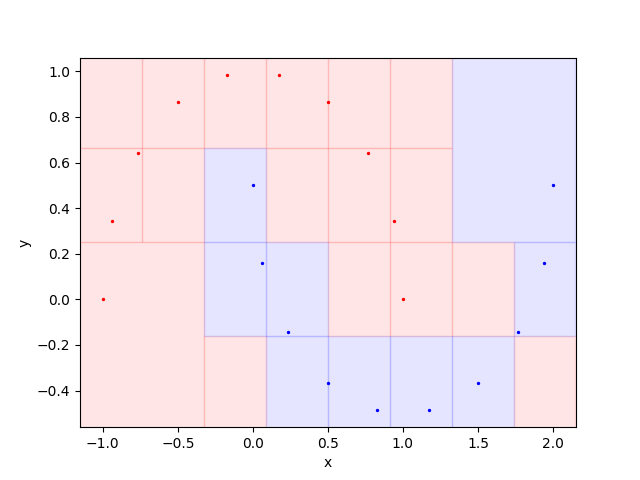
\includegraphics[width=.45\textwidth]{visual20}}\quad
%   \subfloat[][Training Size = 50]{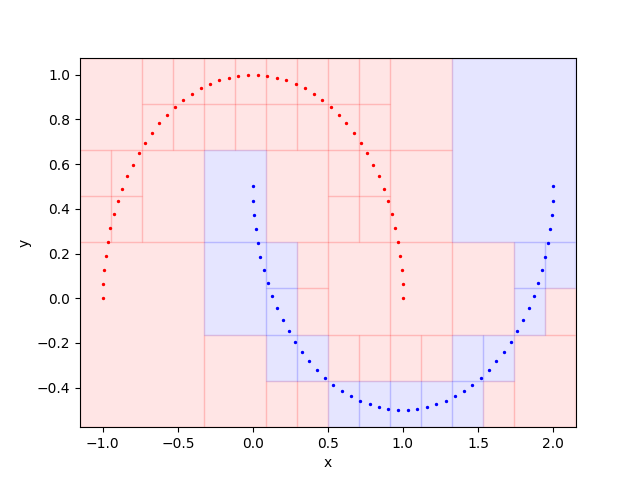
\includegraphics[width=.45\textwidth]{visual50}}\\
%   \subfloat[][Training Size = 500]{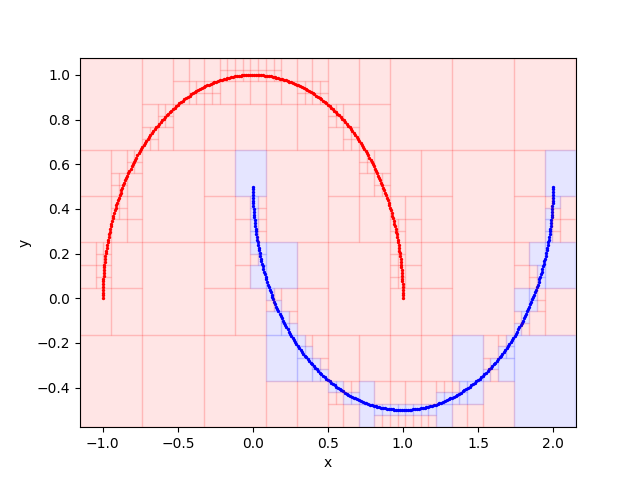
\includegraphics[width=.45\textwidth]{visual500}}\quad
%   \subfloat[][Training Size = 3000]{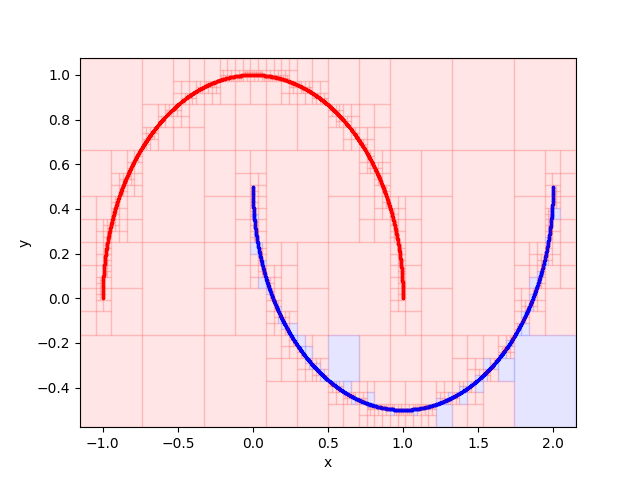
\includegraphics[width=.45\textwidth]{visual3000}}
%\end{center}
%\caption{A visualization of histograms learned with training data sampled from noiseless halfmoon. As training size grows, the histogram classifier becomes increasingly susceptible to adversarial examples in the blue regions.}
%\label{fig:appendix_fig}
%\vskip -0.2in
%\end{figure}

\begin{figure}
\begin{subfigure}{0.45\textwidth}
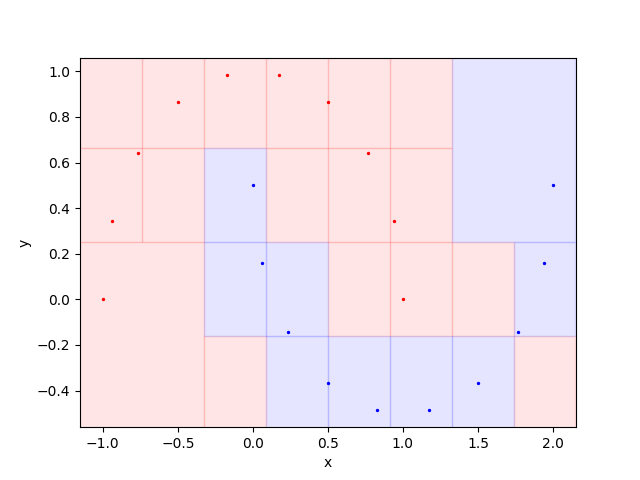
\includegraphics[width=\linewidth]{visual20}
\caption{Training Size = 20} \label{fig:a}
\end{subfigure}\hspace*{\fill}
\begin{subfigure}{0.45\textwidth}
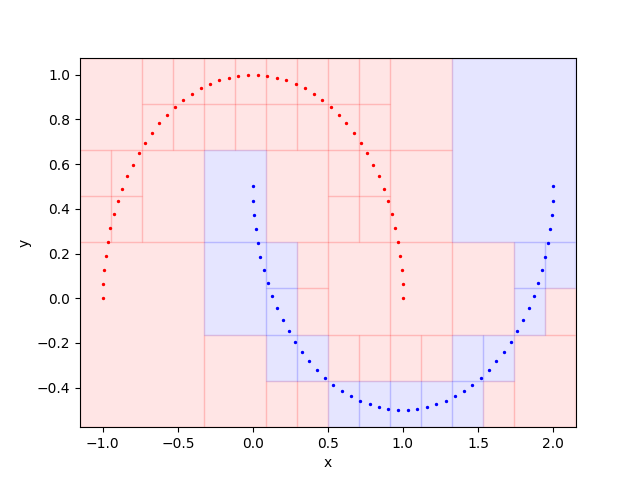
\includegraphics[width=\linewidth]{visual50}
\caption{Training Size = 50} \label{fig:b}
\end{subfigure}

\medskip
\begin{subfigure}{0.45\textwidth}
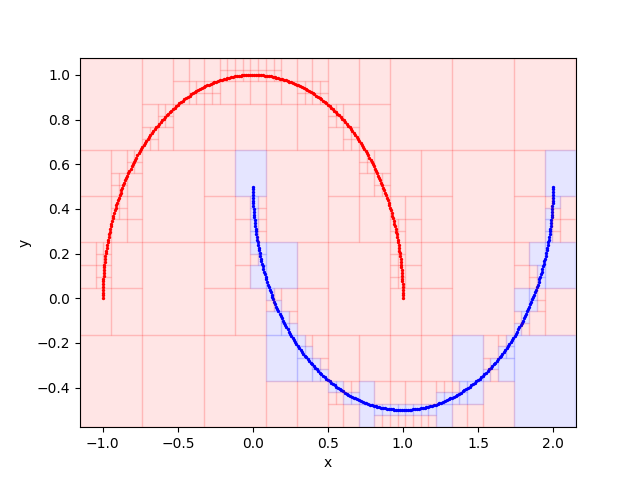
\includegraphics[width=\linewidth]{visual500}
\caption{Training Size = 500} \label{fig:a}
\end{subfigure}\hspace*{\fill}
\begin{subfigure}{0.45\textwidth}
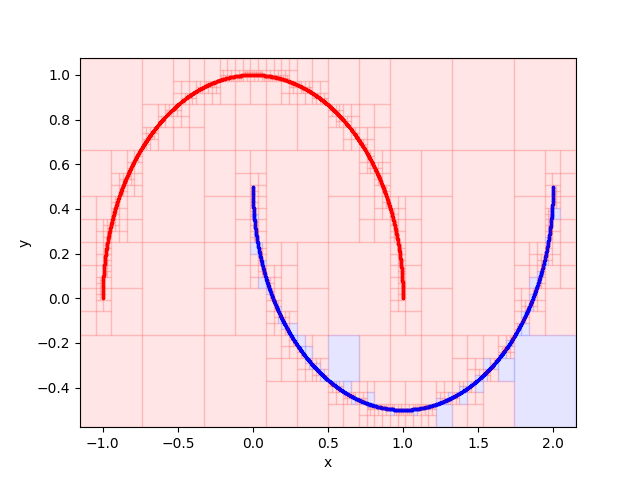
\includegraphics[width=\linewidth]{visual3000}
\caption{Training Size = 3000} \label{fig:b}
\end{subfigure}
%\caption{Sixth subfigure} \label{fig:f}

\caption{Empirical accuracy/astuteness of different classifiers as a function of training sample size. Accuracy is shown in green, astuteness in purple. Left : Noiseless Setting. Right: Noisy Setting. Top Row: Histogram Classifier, Bottom Row: 1-Nearest Neighbor} \label{fig:1}
\end{figure}

\subsection{Optimal attacks against histogram classifiers}

Let $H$ be a histogram classifier, and let $(x,y)$ be any labeled example. Let $r > 0$ be some fixed robustness radius. Recall that an \textit{adversarial example} against $H$ at $(x,y)$ is any $x'$ such that $x' \in B(x,r)$ and $H(x') \neq y$. Note that if $H(x) \neq y$, then $x$ itself is an adversarial example. Conversely, if $H$ is astute at $(x,y)$ with radius $r$, then no adversarial example exists.

For arbitrary classifiers, finding adversarial examples at a given point can be challenging. However, recent work (Yang et. al. 2019) has shown that for non-parametric classifiers, there are tractable methods for doing so. The key insight is that non-parametric classifiers can be construed as a partitioning of input space into convex cells, with each cell having a given label. For example, Figure \ref{fig:appendix_fig} gives a visualization for these cells in a histogram classifier. 

Because these cells are convex, finding an adversarial example for $H$ at $(x,y)$ (here $x$ is a point in $\R^2$, and $y$ is a label) amounts to finding the closest cell $c \in H$ to $x$ such that $H(c) \neq y$. While Yang et. al. (Yang et. al. 2019) presents convex programming algorithms for doing this, the case of histograms in the $\ell_\infty$ metric is much simpler. 

As stated in definition 10, a histogram partitions the input space into hypercubes by iteratively splitting each cube into $2^d$ cubes with half the length. Therefore, the cells of a histogram are all hypercubes of varying sizes. For cell $c$, let $s(c)$ denote the length of the cube that $c$ corresponds to, and let $H(c)$ denote the label $H$ assigns to $c$. The key observation is that $c$ contains an adversarial example for $(x,y)$ if and only if $d(c, x) \leq s(c)/2 + r$, and $H(c) \neq y$. This yields the following algorithm:


Algorithm \ref{alg_hist_attack} was further optimized by utilizing nearest-neighbor type algorithms to find the ``closest" cells to $x$. This was done by grouping cells by their radii, and utilizing a separate nearest-neighbor data structure for all cells of a given radius. 

Although this algorithm doesn't have the same performance metrics as those presented in (Yang et. al. 2019), it was easily sufficient for computing the empirical astuteness for our experiments.

%\begin{algorithm}[tb]
%   \caption{Optimal attack algorithm for Histogram Classifiers}
%   \label{alg_hist_attack}
%\begin{algorithmic}
%   \STATE {\bfseries Input:} Histogram $H$, labeled point $(x,y) \in \R^2 \times \{\pm 1\}$, robustness radius $r$
%   \FOR{cell $c \in H$}
%   \IF{$d(c,x) \leq s(c)/2 + r$ and $H(c) \neq y$}
%   \STATE{Return $c$}
%   \ENDIF
%   \ENDFOR
%\end{algorithmic}
%\end{algorithm}

\begin{algorithm}[H]
    \SetAlgoLined
    {\bfseries Input:} Histogram $H$, labeled point $(x,y) \in \R^2 \times \{\pm 1\}$, robustness radius $r$\;
    
 	\For{cell $c \in H$}{
 		\If{$d(c,x) \leq s(c)/2 + r$ and $H(c) \neq y$}{
 			Return $c$
 		}
 	}
    

\caption{Optimal attack algorithm for Histogram Classifiers}
\end{algorithm}
 